% Stevens NOIR
\documentclass[tikz = true, border = 1pt]{standalone}
\usepackage{amsmath}
\usepackage{amsfonts}
\usepackage{amssymb}
\usepackage{graphicx}
\usepackage{tikz}
\usetikzlibrary{positioning, calc}
\usetikzlibrary{intersections}
\usetikzlibrary{decorations.pathreplacing}
\usetikzlibrary{decorations.text}
\usetikzlibrary{arrows,shapes,backgrounds, shadows,fadings}
\usepackage{fontspec}
\setmainfont{Equity Text A}[SmallCapsFont={Equity Caps A}]
\definecolor{firebrick4}{HTML}{8B1A1A}
\definecolor{royalblue4}{RGB}{39,64,139}
\definecolor{myviolet}{HTML}{51315E}
\begin{document}
	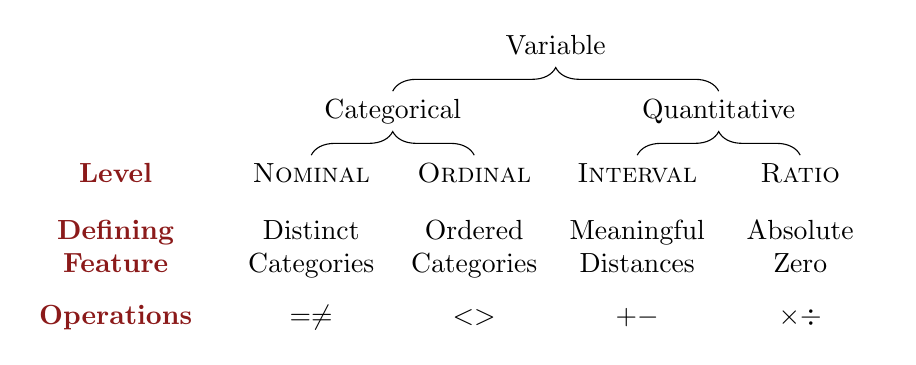
\begin{tikzpicture}[scale=0.9,
	                    text height=1.5ex,
	                    text depth=.25ex,
	                    post/.style={->,
	                                 draw,
	                                 shorten >=4pt,
	                                 shorten <=4pt,
	                                 >=latex',
	                                 very thick,
	                                 font=\large}]
	\node (h) at (2.3, 0) {};
	\node (v) at (0,0.8) {};
	\node (Nominal) at (1, 2) {\textsc{Nominal}};
	\node (Ordinal) at ($(Nominal)+(h)$) {\textsc{Ordinal}};
	\node (Interval) at ($(Nominal)+2*(h)$) {\textsc{Interval}};
	\node (Ratio) at ($(Nominal)+3*(h)$) {\textsc{Ratio}};
	\node [text width=2cm,text centered] (Mutual) at ($(Nominal)-1*(v)$) {Distinct Categories};
	\node [text width=2cm,text centered] (Order) at ($(Ordinal)-1*(v)$) {Ordered Categories};
	\node [text width=2cm,text centered] (Distance) at ($(Interval)-1*(v)$) {Meaningful Distances};
		
	\node [text width=2cm,text centered] (Magnitude) at ($(Ratio)-1*(v)$) {Absolute Zero};

	\node (Equality) at ($(Mutual)-1.5*(v)$) {$=\ne$};
	\node (LessMore) at ($(Order)-1.5*(v)$) {$<>$};
	\node (PlusMinus) at ($(Distance)-1.5*(v)$) {$+-$};
	\node (MultiplyDivide) at ($(Magnitude)-1.5*(v)$) {$\times\div$};
	
	
	\node [color=firebrick4] (Level) at ($(Nominal)-1.2*(h)$) {\textbf{Level}};
	\node [text width=2cm,text centered, color=firebrick4] (Feature) at ($(Level)-1*(v)$) {\textbf{Defining Feature}};
	\node [color=firebrick4] (Operation) at ($(Feature)-1.5*(v)$) {\textbf{Operations}};
	\draw[decoration={brace,amplitude=3mm}, decorate] (Nominal.north) -- (Ordinal.north) node[midway,above=3mm] (Categorical) {Categorical};
	\draw[decoration={brace,amplitude=3mm}, decorate] (Interval.north) -- (Ratio.north) node[midway,above=3mm] (Quantitative) {Quantitative};
	\draw[decoration={brace,amplitude=3mm}, decorate] (Categorical.north) -- (Quantitative.north) node[midway,above=3mm] (Variable) {Variable};
	\end{tikzpicture}
\end{document}
